\documentclass[12pt]{article}
\usepackage{geometry}
\usepackage{fancyhdr}
\usepackage{amsmath, amsthm, amssymb}
\usepackage{graphicx}
\usepackage{hyperref}
\usepackage{array}
\usepackage[table]{xcolor}
\usepackage{rotating}
\usepackage[utf8]{inputenc}
\newcommand{\HRule}{\rule{\linewidth}{0.5mm}}

\usepackage[english]{babel}
\pagestyle{headings}

\begin{document}
\begin{titlepage}
\begin{center}
\thispagestyle{empty}

\textsc{\large Norwegian University of Technology and Science} \\

\vspace{2cm}

\HRule\\[0.5cm]
{\Huge Load Prediction using Hilbert-Huang Transformation}\\[1cm]
\textsc{\large{Smart Grid: Huge Data}}
\HRule\\[3.5cm]

\vspace{5cm}
{\large \emph{By:}}\\
Jonas Eikli\\

\vfill


\end{center}
\end{titlepage}
\newpage


\begin{abstract}
The new Smart Grid is the power grid for the next generation. It is based on the current power grid, but with improvements in every category. One of the main things to improve in the current power grid is the efficiency. With better prediction of power consumption, the efficiency can be increased. This paper tries to answer the question can the Hilbert-Huang Transformation be used for prediction, and specifically, for this kind of prediction. The results show that...


\end{abstract}
\newpage

\subsection*{Preface}
\addcontentsline{toc}{subsection}{Preface}
PREFACE




\newpage
\tableofcontents
\newpage
\listoffigures
\newpage
\listoftables
\newpage
\section{Introduction}
\label{introduction}

The current power grids in use all over the world are inherently inefficient. The main reason for this is that only one third of the fuel is turned into electricity, and the overflow is wasted.  The reason for this inefficiency is that it is designed to withstand maximum load at all times. 20\% of the generation capacity exists to meet peak demands. If the electricity suppliers had more knowledge of how much power was needed, and when it was needed, the waste could be substantially reduced. As we spend more energy, and the resources are starting to dwindle, efficiency is becoming more and more important. This also holds true for areas with limited resources available.

Several other methods exists for predicting, or forecasting, electricity demand. 

The Hilbert-Huang Transform is a method to decompose a signal to get the instantaneous frequency. 

%motivation
%goals
%context
%stakeholders


Research questions:
\begin{enumerate}
\item Can Hilbert-Huang Transformation be used for prediction?
\item Can Hilbert-Huang Transformation be used to predict the load of a power grid?
\end{enumerate}

\section{Power Grid}
\label{powerGrid}
The power grid, or electrical grid, is a vital part of the infrastructure in any country. It serves to transport electricity over great distances, from suppliers to consumers, or from one country to another. While today's power grids certainly are impressive, they are far from perfect. It turns one-third of the fuel into electricity, without recovering the waste. Almost 8\% of its output is lost along the transmission lines, while 20\% of its generation capacity exists to meet peak demand (i.e., it is only in use 5\% of the time) \cite{smartgridPath}.

The power grid is made up from three main components. The \textit{power stations} that produce the electricity, the \textit{transmission lines} that transports the electricity from the suppliers to demand centers, and the \textit{transformers} that reduce voltage so \textit{distribution lines} can deliver it to consumers.

The power stations are usually located away from heavily populated areas. Because of this, a network of power lines are necessary to transport the electricity to where it is needed. This is done first over the transmission lines, then over the distribution lines. On the transmission lines the electricity is transmitted using at high voltages (110kV or above) to reduce the energy lost over long distances. The high voltage electricity is delivered to substations, or transformers, that reduce the voltage and sends the electricity out on the distribution lines. When the power finally arrives at a service location, the voltage is stepped down again, from distribution voltage to the required service voltage. The electricity is then ready for the typical household. 



\subsection{Evolution of the Smart grid}
\label{smartGrid}
The existing power grid is essentially a one-way pipeline where the source have no real-time information about the end points. Because of this, the grid is over-engineered to withstand maximum anticipated peak demand across its aggregated load. Since this is an infrequent occurrence, this system is inherently inefficient. The suppliers need to know, or at least predict, how much power is needed in order to increase efficiency. 

The earliest attempts from the power industry at solving this was the automated meter reading (AMR). AMR let utilities read the consumptions records, alarms and status from customers' premises remotely. While this looked promising at first, it did not solve the major problem, that is, demand-side management. It is limited to reading data, so it can not take corrective action based on the received information. AMR systems do not allow the transition to the smart grid, where pervasive control at all levels is a basic premise \cite{smartgridPath}.

As a consequence of this, AMR was short lived. Instead, the advanced metering infrastructure (AMI) was introduced. Through AMI, utilities get a two-way communication system to the meter, as well as the ability to modify customers' service-level parameters. AMI paved the path for the new smart grid, which is currently under development.

The Smart Grid is a developing network of new technologies, equipment, and controls working together to respond immediately to our 21st century demand for electricity \cite{smartGridGov}. Is is the full range of current and proposed solutions to the challenges of electricity supply. Smart Grid spans many different fields and technologies, including intelligent agents, intelligent applications, network management, distributed control, smart sensors and two-way communication. Some of these are already done by AMI, but the rest are still under development. 

The goals of the Smart Grid is to get a more efficient, more robust, self-healing power grid, that can cope with the increased demand for electricity in years to come.



\section{Hilbert-Huang Transformation}
\label{hilbertHuangTransformation}

The Hilbert-Huang Transformation (HHT) is a way to decompose a signal into intrinsic mode functions (IMF), and obtain instantaneous frequency data. Unlike the Fourier transformation, it is designed to work well for data that are nonstationary and nonlinear. The HHT consists of the empirical mode decomposition (EMD) and the Hilbert Spectral analysis (HSA). The EMD is used to make IMFs and the HSA is used to obtain the instantaneous frequency data.

The EMD consists of a sifting process that is repeated a number of times. The sifting process is as follows:

\begin{enumerate}
\item Find all local extrema, maxima and minima, in the data.
\item Connect all the maxima using a cubic spline line as an upped envelope.
\item Connect all the minima the same way.
\item Calculate a mean between the upper and lower envelope.
\item Subtract the mean from the data.
\item The result of this is used as input in the next sifting.
\end{enumerate}

There are two possible stoppage criteria that can determine how many times the sifting process is repeated. The first is proposed by Huang et al. (1998) and is similar to the Cauchy convergence test. First, a threshold is given, and when the sum of the difference is smaller that the threshold, the sifting process stop. The sum of the difference is defined as: 

\begin{equation}
SD_k=\frac{\sum_{t=0}^{T}|h_{k-1}(t)-h_k(t)|^2}{\sum_{t=0}^{T} h_{k-1}^2 (t)}.\,
\end{equation}

The second possible stoppage criteria is based on the so-called S-number, which is defined as the number of consecutive siftings when the numbers of zero-crossings and extrema are equal or differ at the most by one. The sifting process with only stop when the number of successive siftings where this is true reaches the pre-selected S-number. Huang et al. (2003) suggests that the optimal range for S lies between 3 and 8. 

When the stoppage criterion is met, the first IMF is created. This IMF is removed from the original data by subtracting it, and the result is the residue. The first IMF contains the finest scale, or the shortest period component of the signal, and the residue is left with longer period variations in the data.

The whole procedure is repeated with the residue as input. This is done until the residue becomes a monotonic function from which no IMF can be extracted. 


\section{Artificial Neural Networks}
\label{ann}
An artificial neural network (ANN) is a mathematical model inspired by biological neural networks. The ANN consists of several layers; the input layer, one or more hidden layers, and the output layer. Each layer has one or more artificial neurons. The neurons in the different layers are connected by weighted edges. An example of an ANN, with 4 input neurons, 5 hidden neurons and 2 output neruons, can be seen in Figure \ref{fig:ann}. Each neuron also has an activation function that determines if it is activated or not. The activation level is based on the input and determines the output of the neuron. An ANN is typically defined by three types of parameters:

\begin{figure}[h]
\centering
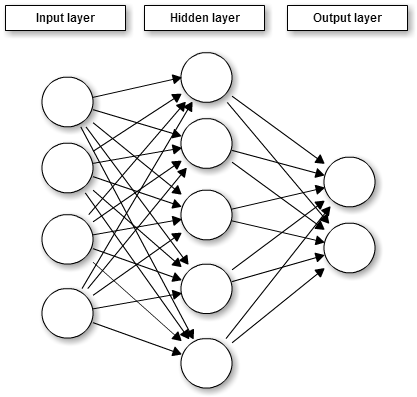
\includegraphics[width = 0.6\textwidth]{ann}
\caption{A typical feedforward ANN}
\label{fig:ann}
\end{figure}

\begin{enumerate}
\item The interconnection pattern between different layers of neurons.
\item The learning process for updating the weights of the interconnection.
\item The activation function that converts a neuron's weighted input to its output activation.
\end{enumerate}

There are three different paradigms for training ANNs, these are:

\begin{description}
\item \textbf{Supervised Learning} \hfill \\
When using supervised learning, the network is provided with both sample inputs, as well as the desired outputs for each case. The well-known \textit{backpropagation} algorithm can be used for training. Typical tasks solved by this paradigm is pattern recognition and regression. 
\item \textbf{Unsupervised Learning} \hfill \\
In unsupervised learning, the desired output is not given, so the goal is typically to minimize the cost function for the input data. Typical tasks here are general estimation problems.
\item \textbf{Reinforcement Learning} \hfill \\
In reinforcement learning, the input data is typically not given. The aim is to discover a policy for selection actions that minimize some measure of long-term cost. Typical applications for reinforcement learning are control problems like for example games. 
\end{description}

For the task in this project, supervised learning is the obvious paradigm to use.

Based on the structured literature search in Appendix \ref{SLR}, the neural network that will be used in this project is the General Regression Neural Network, discussed in Section \ref{grnn}.

\subsection{General Regression Neural Network and the Radial Basis Function}
\label{grnn}
The General Regression Neural Network (GRNN)\cite{grnn} is a type of Radial Basis Function (RBF) network. The difference being that GRNN have one input neuron for each point in the training set, whereas RBF networks have a variable number of neurons that are usually lower than the number of training points.

GRNN are conceptually similar to K-Nearest Neighbour models. When predicting the target value of some input, the idea is that the target value should be close to output from similar input generated during training. That is, similar input gives similar output. To decide which of the neighbours is to be used for determining output, they are weighted based on the distance from the point in question. The weight is decided using the Radial Basis Function. Different types of RBFs can be used, but the most common is the Gaussian function. 

The GRNN also uses a smoothing parameter $\sigma$. A large $\sigma$ will result in a large spread Gaussian and the sample points will cover a wide range of inputs, while a small value will create a limited spread Gaussian and the sample points will cover a small range of inputs. It is important to find a good value for $\sigma$, so that it will cover up any noise, while at the same time not smoothing over important features. With a higher number of test cases, a lower value for $\sigma$ can be used. 

GRNN has several advantages over other non-linear regression techniques\cite{grnn}: 
\begin{enumerate}
\item The network is trained by one pass through the data and can generalize from examples as soon as they are stored.
\item The estimate converges to the conditional mean regression surface as more and more examples are observer, yet it can form a very reasonable regression surface based on only few examples.
\item The estimate is bounded by the minimum and maximum of the observations.
\item The estimate does not converge to poor solutions corresponding to local minima or maxima. 
\item Its easy to use.
\item The network can provide a mapping from one set of sample points to another. If this is one-to-one, it can be easily reversed. 
\end{enumerate}

The neural network in a GRNN consist of 4 layers; the input layer, the hidden layer, the pattern layer/summation layer and the decision layer. The input layer has one neuron for each predictor variable. The hidden layer has one neuron for each case in the training set. In the pattern layer, there are two neurons, one is the denominator summation unit and the other is the numerator summation unit. The decision layer has one node which divides the value accumulated in the numerator summation unit by the value in the denominator summation unit and uses the result as the predicted output value. 

Let us consider a case where there is one input value and N training cases. This network would have 1 neuron in the input layer, N neurons in the hidden layer, two in the pattern layer and one in the decision layer. This GRNN can be seen in Figure \ref{fig:grnn}.

\begin{figure}[h]
\centering
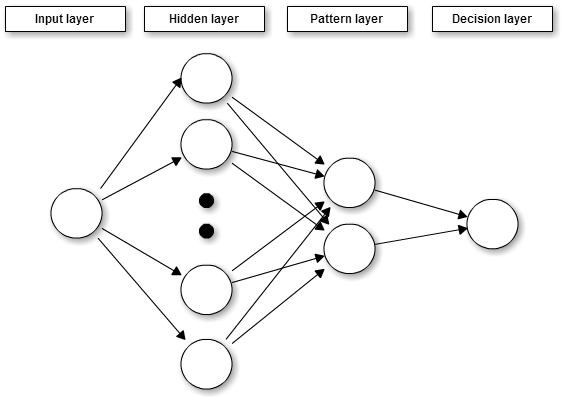
\includegraphics[width = 0.7\textwidth]{grnn}
\caption{A general regression neural network with one input value and N training cases.}
\label{fig:grnn}
\end{figure}


\section{Implementation}
\label{implementation}
This section will reason for of the decisions made during this project, and try to explain why things have been done a certain way. Section \ref{python} discusses why Python selected as the programming language to use, as well as which libraries were used. Section \ref{prediction} discusses the method used for prediction and why that was selected.

\subsection{Power Grid}
\label{powergrid}
The data used in this project is from a database provided by the advisor. The data is collected over a period of 6 years from a distribution network in Canada. Because it is from a distribution network, there is very little noise in the data, as the distribution network provides power to a lot end users. This results in a very good signal, that clearly shows each day. A section of this signal can be seen in Figure \ref{fig:10days}. This figure shows 10 days. It is easy to see the days, with peaks in the morning and evenings, and low points at night and during the day when people are at work. A lot more power is consumed during the days in the middle of the graph. Why this is, can be hard to say. The most likely reason is that there was cold weather during this period, or it might be a weekend.

\begin{figure}[h]
\centering
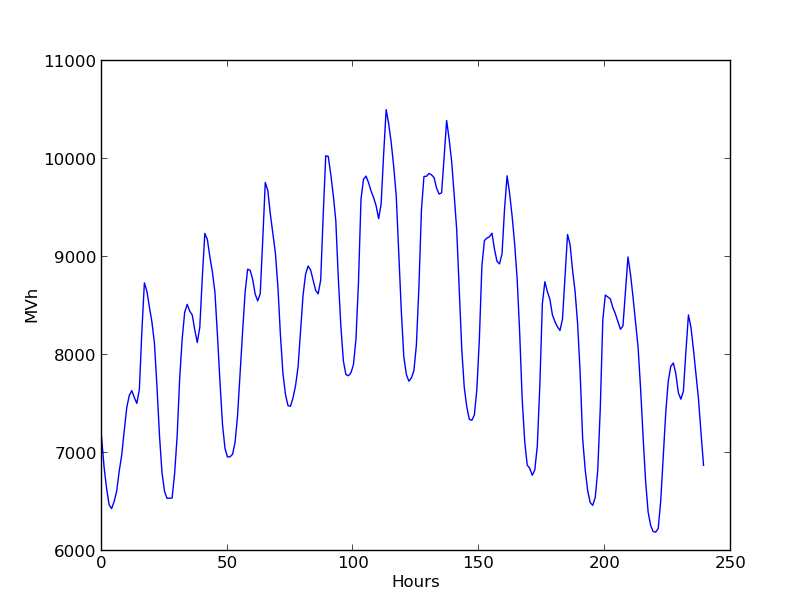
\includegraphics[width = \textwidth]{10days}
\caption{10 days of power consumption}
\label{fig:10days}
\end{figure}




\subsection{Python}
\label{python}
Python\footnote{http://www.python.org/} is a general purpose, interpreted high-level programming language. The reasons for choosing Python as programming language in this project are:

\begin{itemize}
\item Pre-existing code for retrieving data from the database containing power consumption data. 
\item Python is easy to use, and easy to get started with. It's ideal for systems of this scale.
\item Libraries containing useful code, as discussed below.
\item Using Python was recommended from the advisor. 
\item Python, as well as most of the libraries, are free.
\end{itemize}

One of the main reasons for using Python is that there are many libraries, or packages or modules, available to make things easier. The, not already included in Python, libraries  used in this project is described below:

\begin{description}
\item \textbf{NumPy\footnote{http://numpy.scipy.org/}} \hfill \\
NumPy is the fundamental package for scientific computing with Python. It provides Python with a host of both simple and advanced mathematical functionality. It is required for using SciPy.
\item \textbf{SciPy\footnote{http://www.scipy.org/}} \hfill \\
SciPy is another package for scientific computing. It provides modules for, among other things, statistics, optimization, numerical integration, signal processing and Fourier transforms. In this project, it is used for finding the spline functions used when finding maxima and minima in HHT, as well as in the Hilbert transform.
\item \textbf{Pandas\footnote{http://pandas.pydata.org/}} \hfill \\
Pandas is a library that provides Python with high-performance, easy-to-use data structures and data analysis tools. The power consumption data from the database was stored in Pandas time series.
\item \textbf{MatPlotLib\footnote{http://matplotlib.org/}} \hfill \\
MatPlotLib is a powerful library used for plotting 2D graphs. It is used to plot all the graphs in this report.
\item \textbf{Peach\footnote{http://pypi.python.org/pypi/Peach/0.3.1}} \hfill \\
Peach is a module based on SciPy and NumPy used to implement algorithms for computational intelligence and machine learning. The ANN used in this project is implemented using Peach. The ANN is discussed further in Section \ref{prediction}.
\end{description}

\subsection{Hilbert-Huang Transform}
\label{hht}
HHT is used in this project to find input variables for the prediction method. Why this is done should be obvious, as this is the very reason for the project. However, as HHT generates many IMFs as output, and each IMF has a instantaneous frequency and amplitude, there is the question of which of these to choose as input to the ANN. From the literature, it is clear that there are many ways to do this, but a mix of IMFs, frequencies and amplitudes tends to perform very well. This is something that needs to be experimented on, to see what gives the best results. 


\subsection{Prediction}
\label{prediction}
The decision the use an artificial neural network (ANN) for prediction is based on the results of the structured literary review, Appendix \ref{SLR}. From the articles found there, it was clear that ANN is a widely used method of prediction when dealing with time series, and it also gives the best results. 

Of the ANNs used in the literature, the general regression neural network (GRNN) was selected as the one to be used in this project. The other ANNs discussed was Multilayer Perceptron (MLP) and Radial Basis Function Network. Because of time constraints, only one was implemented. The reason for choosing GRNN was that, according to the literature, it gave very good results. Additionally, the Peach library for Python has methods for implementing a GRNN, so that saves a lot of time.

The GRNN was implemented using the Peach package. 

\section{Results}
\label{results}



\section{Discussion}
\label{discussion}



\section{Conclusion}
\label{conclusion}




\section{Future Work}
\label{futureWork}

end point optimization in HHT

radial basis function

multilayer perceptron

more work on which parameters to use as input

more robust

how will it do with a lot of noise

how weather impacts things

\section{Project evaluation}
\label{projectEvaluation}




\newpage
\bibliographystyle{plain}
\bibliography{Bibliography}


\appendix


%\documentclass[12pt]{article}

%\begin{document}
\section{Systematic Literary Review}
\label{sec:SLR}

This is the full version of the systematic literary research. It describes how and where the sources used in this project can be found, as well as the rationale for selecting the sources that are used. The reason for including a systematic literary review is to help the reader understand why certain articles are included, while others are not. 



\subsection{Sources}
\label{sec:sources}



\begin{table}[h]
\centering
\begin{tabular}{|l|}
\hline
\textbf{Source}\\ \hline
IEEE Xplore\\ \hline
SpringerLink\\ \hline
Scopus\\ \hline
\end{tabular}
\caption{Databases used for literary search}
\label{tab:sources}
\end{table}

Table \ref{tab:sources} show the databases used for finding the articles cited in this project. The reasons for choosing these databases is that they are very popular and reliable, especially in the fields related to this project.


\subsection{Search Terms}
\label{sec:searchterms}

\begin{table}[h]
\centering
\begin{tabular}{|l|p{3cm}|l|l|l|}
\hline
 					& \textbf{Group 1} 			& \textbf{Group 2} 	& \textbf{Group 3} 	& \textbf{Group 4}	\\ \hline
\textbf{Term 1} 	& Hilbert Huang Transform 	& Forecast			& Time series		& Smart Grid		\\ \hline
\textbf{Term 2} 	& HHT 						& Prediction		& 					& Power Grid		\\ \hline
\textbf{Term 3} 	& 							& Forecasting		& 					& Electrical Grid	\\ \hline
\end{tabular}
\caption{Phrases used when searching}
\label{tab:keywords}
\end{table}

When searching for literature related to this project, the search phrases in Table \ref{tab:keywords} was used. They were put together in a search string in an attempt to get only relevant articles. The phrases was combined like this (T being the term, and G being the group):

\[([G1,T1]\vee[G1,T2])\land  ([G2,T1]\vee[G2,T2]\vee[G2,T3])\land ([G3,T1]) \land ([G4,T1]\vee[G4,T2]\vee[G4,T3])   \]

However, this resulted in only one hit in the databases. This is far from enough, so the search was repeated without Group 4. This gave better results, while still being relevant. 

\subsection{Research Questions}
\label{sec:researchquestions}
\begin{table}[h]
\centering
\begin{tabular}{|l|p{12cm}|} \hline
RQ1	& Can Hilbert-Huang Transform (HHT) be used for load forecasting? \\ \hline
RQ2	& How can the HHT be use for prediction? \\ \hline
RQ3	& Does using HHT for prediction offer any improvements over other methods of prediction? \\ \hline
\end{tabular}
\caption{Research questions}
\label{tab:researchquestions}
\end{table}

The research questions in Table \ref{tab:researchquestions} are the questions that the report will try to answer. RQ1 is really the reason for doing the project, more than a research question. It is still included in the table, as it is something that hopefully will be answered by the project.

\subsection{Inclusion Criteria}
\label{sec:inclusioncriteria}
\begin{table}[h]
\centering
\begin{tabular}{|l|p{12cm}|} \hline
IC1 & The article's main concern is using HHT for prediction.\\ \hline
IC2 & The article describes how and why HHT was used\\ \hline
IC3 & The article compares HHT to other methods for prediction\\ \hline
IC4 & The article has empirical proof, or cites another article, when making statements\\ \hline
\end{tabular}
\caption{Inclusion criteria}
\label{tab:inclusioncriteria}
\end{table}

The articles that got selected from the search results was selected using the inclusion criteria found in Table \ref{tab:inclusioncriteria}. IC1 was of course the most important inclusion criteria. All articles selected had to, at least, fulfil that one, as well as one or more of the other criteria.


\subsection{Quality Assessment}
\label{sec:qualityassessment}
\begin{table}[h]
\centering
\begin{tabular}{|l|l|} \hline
QC1 & The study is put into context of other studies\\ \hline
QC2 & The aim of the research is clearly stated\\ \hline
QC3 & Decisions made are clearly justified\\ \hline
QC4 & The results and procedures are thoroughly explained and analysed \\ \hline
QC5 & The article is structured and uses good language \\ \hline
\end{tabular}
\caption{Quality criteria}
\label{tab:qualitycriteria}
\end{table}

The articles that got selected using the inclusion criteria described, are rated using the quality criteria from Table \ref{tab:qualitycriteria}. Each article got a score (0, 0.5 or 1) for each quality criteria. The scores where summed up, and the ones with the highest scores were considered the best articles, and were given the most weight when doing this project.


\subsection{SLR Results}
\label{sec:slrresults}
This section describes the results achieved from doing the structured literary review described in Section \ref{sec:SLR}. Section \ref{sec:description} briefly describes all the selected articles from Section \ref{sec:literature}. A summary is found in Section \ref{sec:summary}.

\subsubsection{Literature Found}
\label{sec:literature}
\begin{table}[h]
\centering
\begin{tabular}{|l|p{12cm}|} \hline
A1 & Short term wind power forecasting using Hilbert-Huang Transform and artificial neural network\cite{annForecastingModel}\\ \hline
A2 & The hybrid model based on Hilbert-Huang Transform and neural networks for forecasting of short-term operation conditions of power system\cite{hhtTransformModel}\\ \hline
A3 & On the neural network approach for forecasting of non-stationary time series on the basis of the Hilbert-Huang transform\cite{neuralNetAproach}\\ \hline
A4 & Electricity prices neural networks forecast using the Hilbert-Huang transform\cite{electricityPrices} \\ \hline
A5 & Boundary processing of HHT using support vector regression machines\cite{boundaryProcessing} \\ \hline
A6 & Filter principle of Hilbert-Huang transform and its application in time series analysis\cite{filter} \\ \hline
A7 & A new short-term load forecasting model of power system based on HHT and ANN \cite{powersystem}\\ \hline
\end{tabular}
\caption{The articles selected in the SLR, using the key words from Table \ref{tab:keywords} and inclusion criteria from Table \ref{tab:inclusioncriteria}}
\label{tab:articles}
\end{table}

Table \ref{tab:articles} shows the articles that were selected, using the inclusion criteria, from the larger set of articles return from doing the search. Addition information about the articles can be found in the bibliography.

\subsubsection{Description of Articles}
\label{sec:description}

\begin{table}[h]
\centering
\begin{tabular}{|l|l|l|l|l|l|l|} \hline
Article & QC1 	& QC2 	& QC3 	& QC4 	& QC5 	& SUM \\ \hline
A1 		& 1 	& 1 	& 1 	& 0.5 	& 0.5 	& 4\\ \hline
A2 		& 1 	& 0.5 	& 1 	& 1 	& 1 	& 4.5\\ \hline
A3 		& 0.5 	& 0 	& 1 	& 1 	& 1 	& 3.5\\ \hline
A4 		& 1 	& 1 	& 0 	& 0 	& 1 	& 3\\ \hline
A5 		& 1 	& 1 	& 0.5 	& 0.5 	& 1 	& 4\\ \hline
A6 		& 0.5	& 1 	& 1 	& 0.5 	& 1 	& 4\\ \hline
A7 		& 1 	& 1 	& 1 	& 0.5 	& 1 	& 4.5\\ \hline
\end{tabular}
\caption{Quality criteria scores for the selected articles}
\label{tab:qcscore}
\end{table}


The scores each article got for each quality criteria can be seen in Table \ref{tab:qcscore}. Most articles scored quite good, with the exception of A4, which only got a total score of 3. A brief description of each article follows.

\begin{description}
\item A1 \hfill \\
This paper describes how HHT and Artificial Neural Networks (ANN) can be used for forecasting the power generated by wind power. The paper proposes an HHT-ANN model for wind power forecasting, and analyses a case study of a wind farm in Texas to find its results. The conclusion is that the proposed HHT-ANN model is suitable for short-term wind power output forecasting. 
\item A2 \hfill \\
This paper addresses the conventional approaches to the short-term forecasting of non-stationary processes in complex power systems using ANNs. It asks the question if preprocessing of the data can significantly improve the forecast. The focus of the article is HHT, and using that as a means for preprocessing. The conclusion is that using ANN for preprocessing gives better result that no preprocessing. 
\item A3 \hfill \\
This article proposes a two-stage adaptive approach for time series forecasting. The two stages are decomposition of the original time series using Hilbert Transform, and the second is using the obtains functions, as well as instantaneous amplitudes as input in a neural network. The article concludes that the use of HHT permits increasing the accuracy of forecasting. 
\item A4 \hfill \\
The focus of this article is the problem of forecasting of electricity prices. The paper proposes an ``intelligent'' approach which supposes the use of neural network technology together with HHT. The conclusion is that the use of the ``intelligent'' approach increases the accuracy of forecasting, and that the error of short term forecasting is decreased. It is not clear what it is compared against. 
\item A5 \hfill \\
This article focuses on how to restrain the end effects in HHT. Support Vector Regression Machines (SVRM) that are adopted to extend the data at both ends of a signal, is proposed as a solution. Particle Swarm Optimization (PSO) is proposed used for optimizing parameters. The conclusion is that experiments show that the end effects in HHT can be restrained effectively by this method, and that SVRM is a suitable forecasting method for time series. 
\item A6 \hfill \\
This paper puts forward a smoothing filter theory for explaining Empirical Mode Decomposition (EMD) in HHT. HHT is promoted for providing higher resolution and concentration in time-frequency plane and for avoiding false high frequency and energy dispersion. The schemed method is validated through experiments. 
\item A7 \hfill \\
This article proposes a new short-term load forecasting model based on HHT and ANN. The article discuss disadvantages of using HHT for forecasting. The article concludes that, through using the new model, a higher accuracy of short term forecasting can be achieved.

\end{description}




\subsubsection{Summary}
\label{sec:summary}

After reading the articles in Table \ref{tab:articles}, it is pretty clear that HHT can indeed be used for prediction, or forecasting. At least together with some other form for training algorithm. With the exception of article A5 and A6, all the articles dealt with using HHT and ANN for forecasting. A5 mentions using PSO and SVRM, but considering the overwhelming majority of articles that uses ANN, the latter will be considered the best option when doing the project. 

According to several of the articles HHT is used to create the input to the ANNs. That is, both intrinsic mode functions (IMFs) and instantaneous frequencies and amplitudes are generated from HHT and used in an ANN. 

Using this approach also gives increased performance over various other approaches, like using no preprocessing at all.


%\newpage
%\bibliographystyle{plain}
%\bibliography{Bibliography}


%\end{document}




\end{document}
